\subsubsection{35 Zernike modes datasets clusters densities}
		
		\begin{figure*}[ht!]
			\centering
			\subfloat[4KMeans for Zernike coefficients]{%
				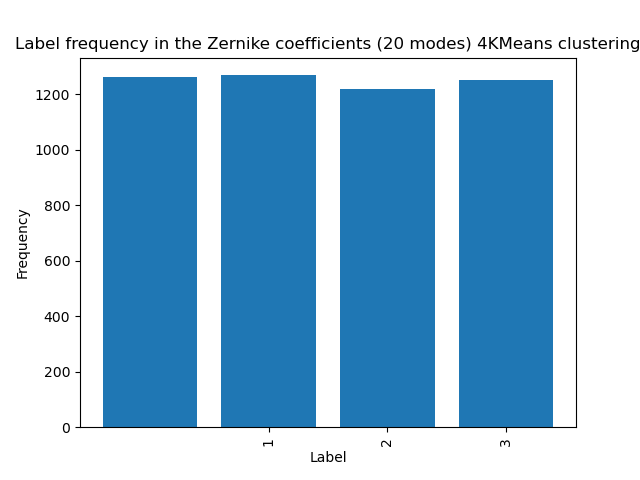
\includegraphics[width=0.2\textwidth]{nmia-zernikecoefficients(20modes)4KMeansdensity.png}}
			\hspace{\fill}
			\subfloat[4KMeans PSF Intensities UMAP]{%
				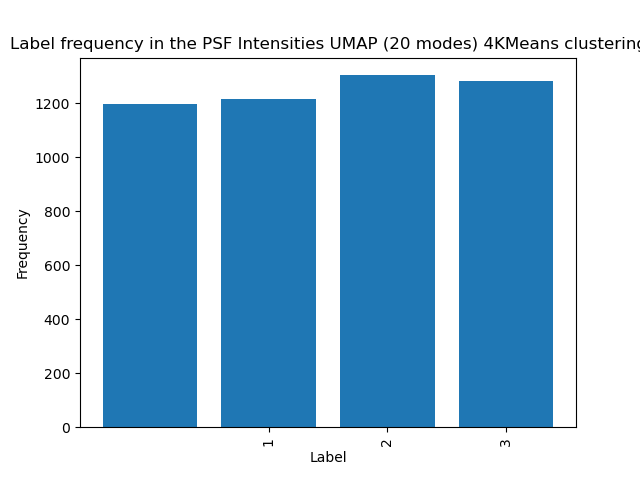
\includegraphics[width=0.2\textwidth]{nmia-psfintensitiesumap(20modes)4KMeansdensity.png}}
			\hspace{\fill}
			\subfloat[4KMeans LP coefficients]{%
				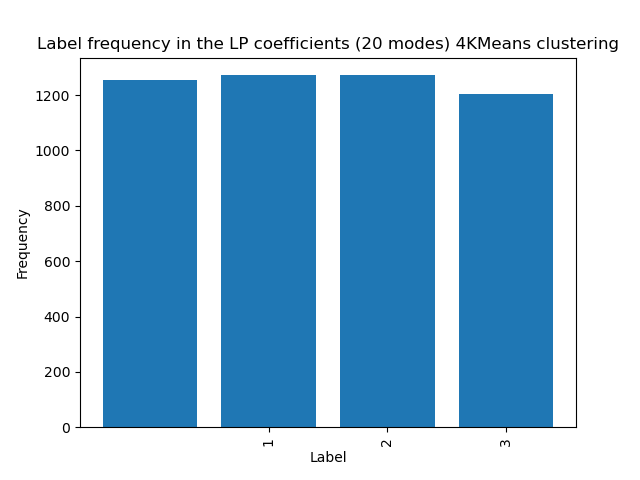
\includegraphics[width=0.2\textwidth]{nmia-lpcoefficients(20modes)4KMeansdensity.png}}
			\hspace{\fill}
			\subfloat[4KMeans Output Fluxes]{%2727
				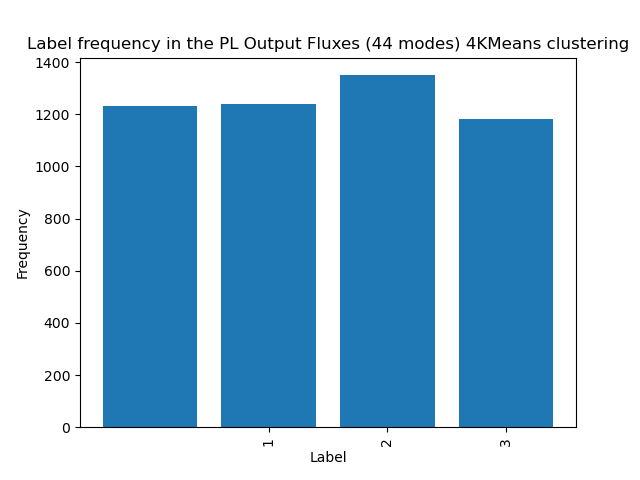
\includegraphics[width=0.2\textwidth]{nmia-ploutputfluxes(44modes)4KMeansdensity.png}}
		\end{figure*}
			
		\begin{figure*}[ht!]
			\centering	
			\subfloat[8KMeans for Zernike coefficients]{%
				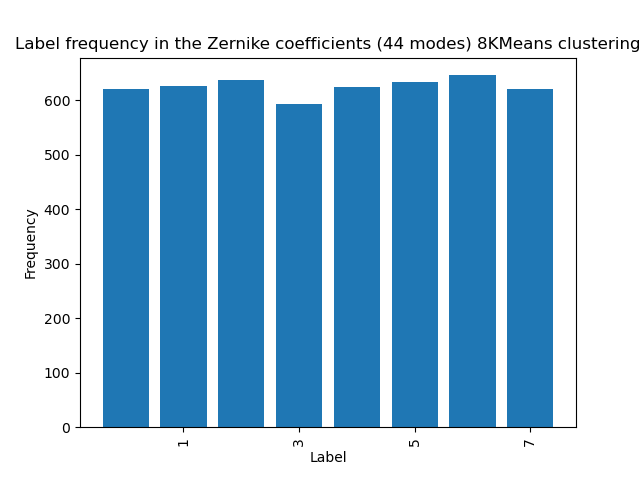
\includegraphics[width=0.2\textwidth]{nmia-zernikecoefficients(44modes)8KMeansdensity.png}}
			\hspace{\fill}
			\subfloat[8KMeans PSF Intensities UMAP]{%
				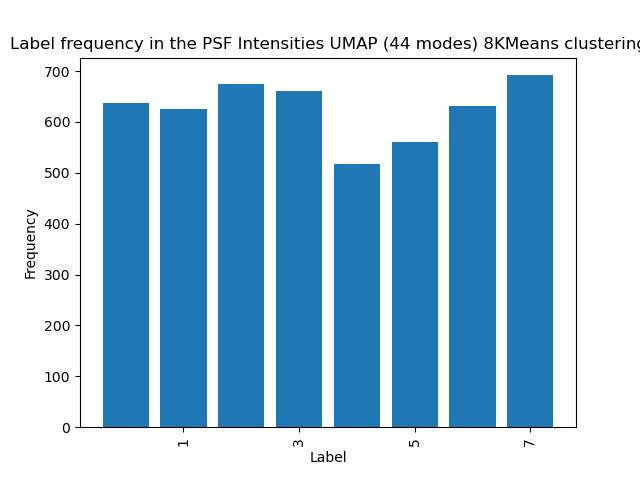
\includegraphics[width=0.2\textwidth]{nmia-psfintensitiesumap(44modes)8KMeansdensity.png}}
			\hspace{\fill}
			\subfloat[8KMeans LP coefficients]{%
				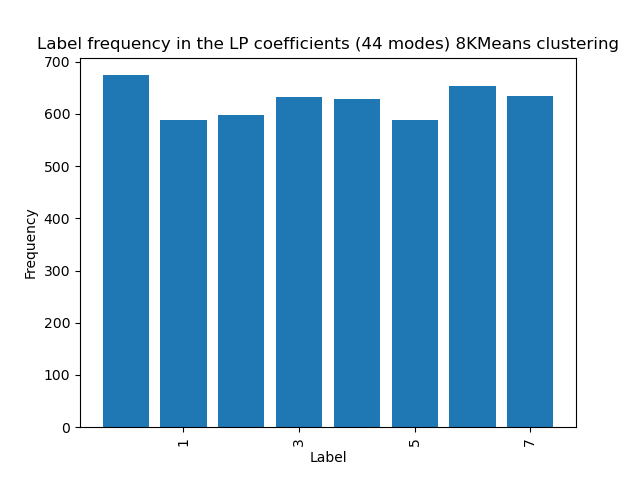
\includegraphics[width=0.2\textwidth]{nmia-lpcoefficients(44modes)8KMeansdensity.png}}
			\hspace{\fill}
			\subfloat[8KMeans Output Fluxes]{%
				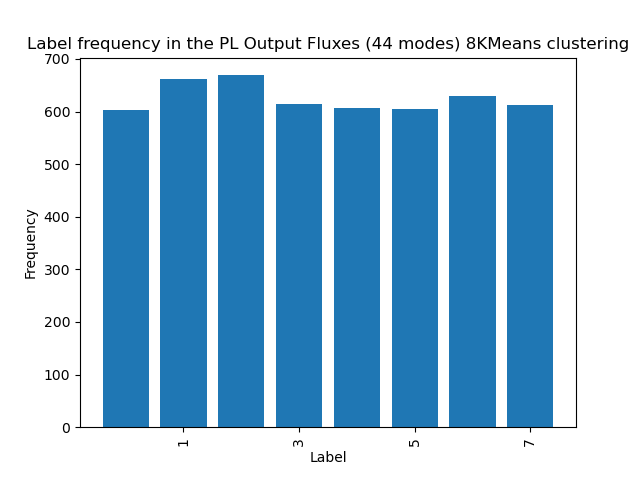
\includegraphics[width=0.2\textwidth]{nmia-ploutputfluxes(44modes)8KMeansdensity.png}}
		\end{figure*}
			
		\begin{figure*}[ht!]
			\centering	
			\subfloat[16KMeans for Zernike coefficients]{%
				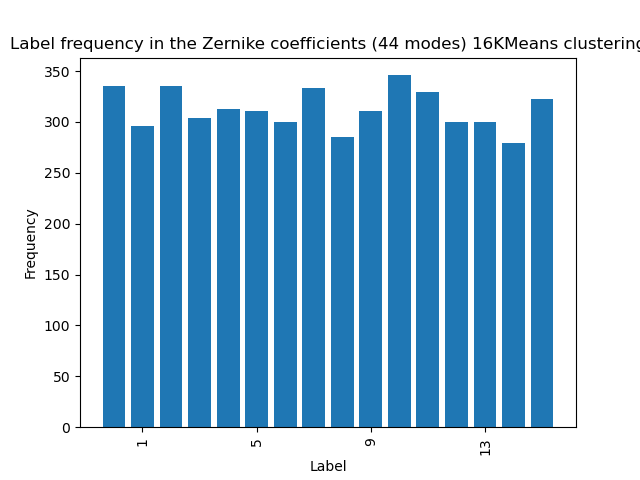
\includegraphics[width=0.2\textwidth]{nmia-zernikecoefficients(44modes)16KMeansdensity.png}}
			\hspace{\fill}
			\subfloat[16KMeans PSF Intensities UMAP]{%
				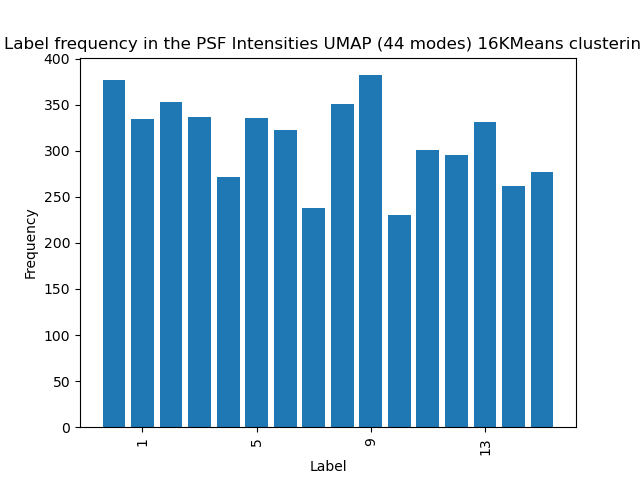
\includegraphics[width=0.2\textwidth]{nmia-psfintensitiesumap(44modes)16KMeansdensity.png}}
			\hspace{\fill}
			\subfloat[16KMeans LP coefficients]{%
				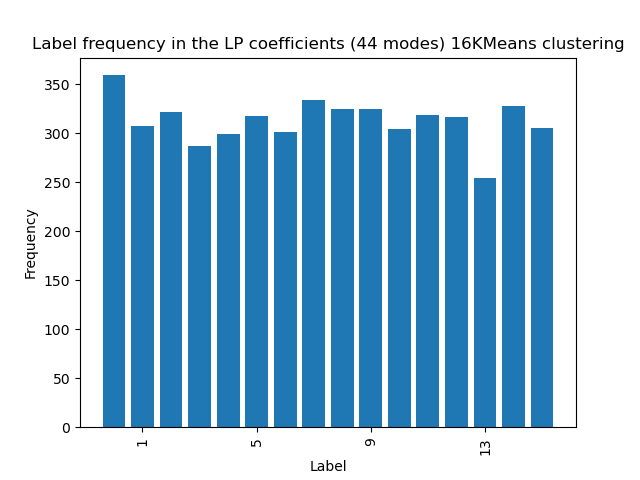
\includegraphics[width=0.2\textwidth]{nmia-lpcoefficients(44modes)16KMeansdensity.png}}
			\hspace{\fill}
			\subfloat[16KMeans Output Fluxes]{%
				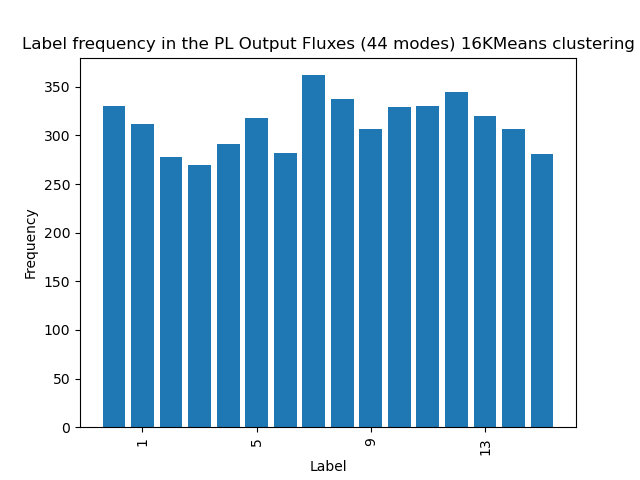
\includegraphics[width=0.2\textwidth]{nmia-ploutputfluxes(44modes)16KMeansdensity.png}}
		\end{figure*}
			
		\begin{figure*}[ht!]
			\centering
			\subfloat[32KMeans for Zernike coefficients]{%
				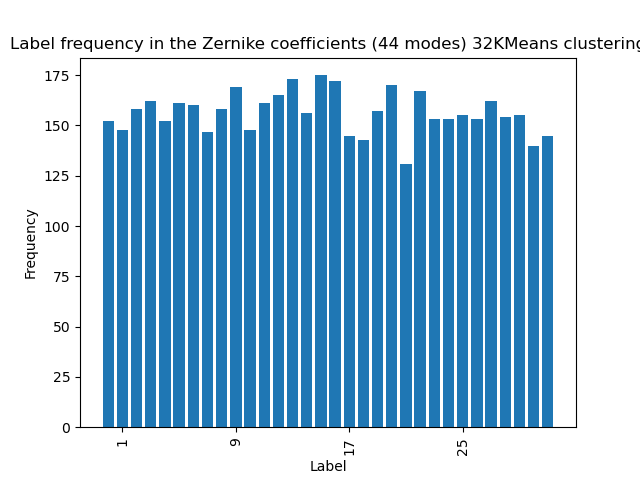
\includegraphics[width=0.2\textwidth]{nmia-zernikecoefficients(44modes)32KMeansdensity.png}}
			\hspace{\fill}
			\subfloat[32KMeans PSF Intensities UMAP]{%
				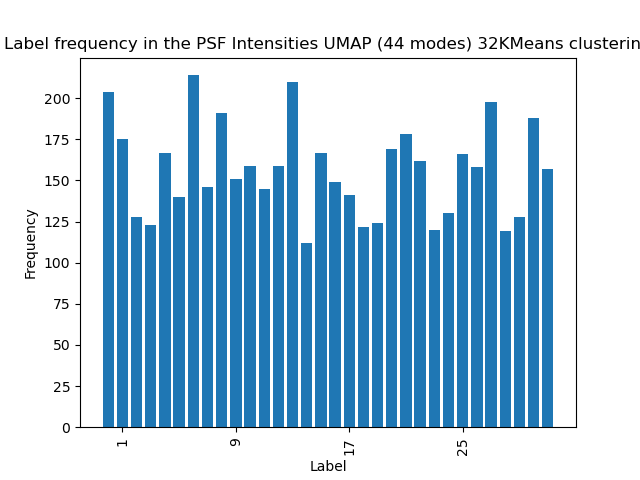
\includegraphics[width=0.2\textwidth]{nmia-psfintensitiesumap(44modes)32KMeansdensity.png}}
			\hspace{\fill}
			\subfloat[32KMeans LP coefficients]{%
				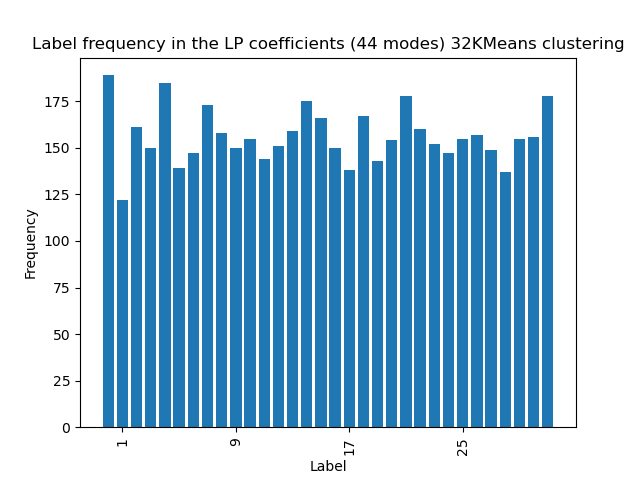
\includegraphics[width=0.2\textwidth]{nmia-lpcoefficients(44modes)32KMeansdensity.png}}
			\hspace{\fill}
			\subfloat[32KMeans Output Fluxes]{%
				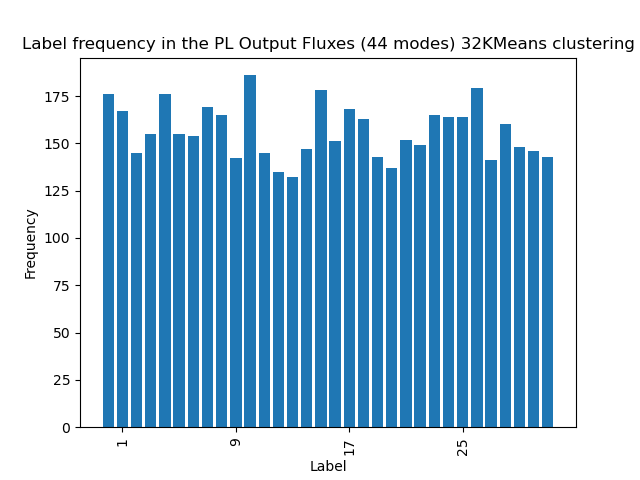
\includegraphics[width=0.2\textwidth]{nmia-ploutputfluxes(44modes)32KMeansdensity.png}}
		\end{figure*}
			
		\begin{figure*}[ht!]
			\centering	
			\subfloat[64KMeans for Zernike coefficients]{%
				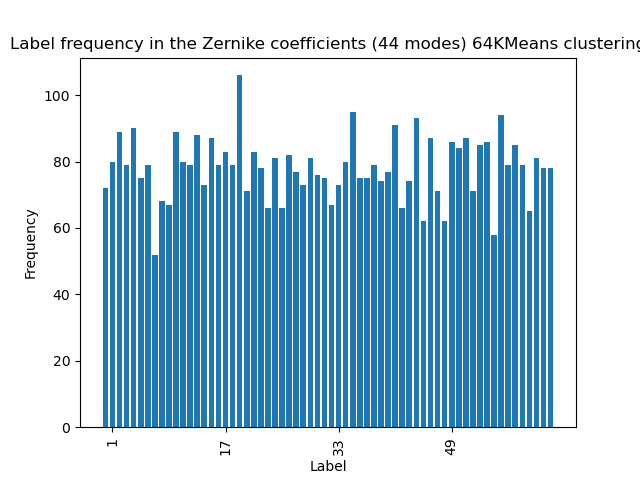
\includegraphics[width=0.2\textwidth]{nmia-zernikecoefficients(44modes)64KMeansdensity.png}}
			\hspace{\fill}
			\subfloat[64KMeans PSF Intensities UMAP]{%
				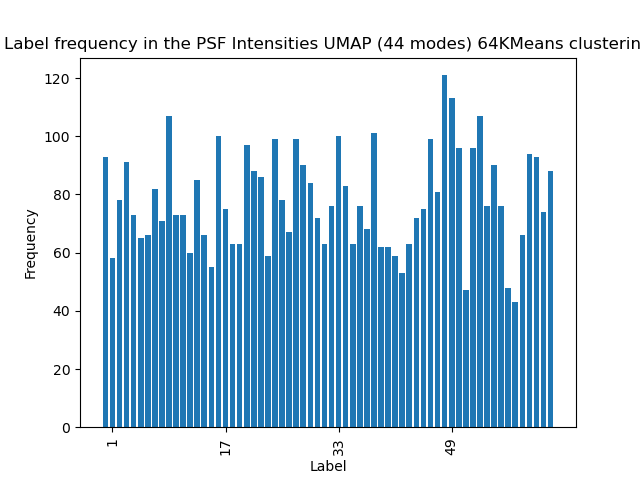
\includegraphics[width=0.2\textwidth]{nmia-psfintensitiesumap(44modes)64KMeansdensity.png}}
			\hspace{\fill}
			\subfloat[64KMeans LP coefficients]{%
				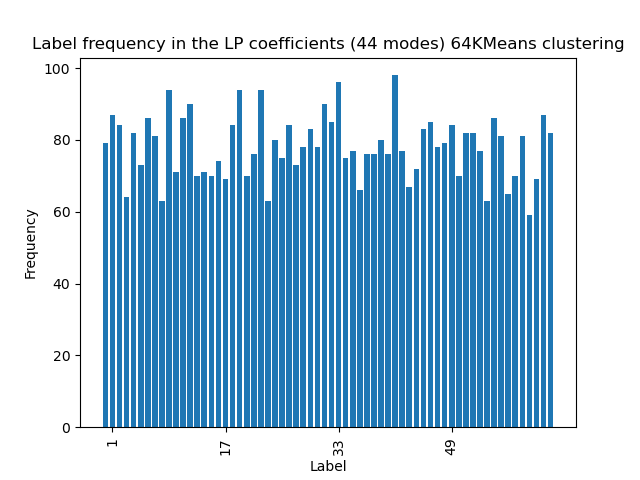
\includegraphics[width=0.2\textwidth]{nmia-lpcoefficients(44modes)64KMeansdensity.png}}
			\hspace{\fill}
			\subfloat[64KMeans Output Fluxes]{%
				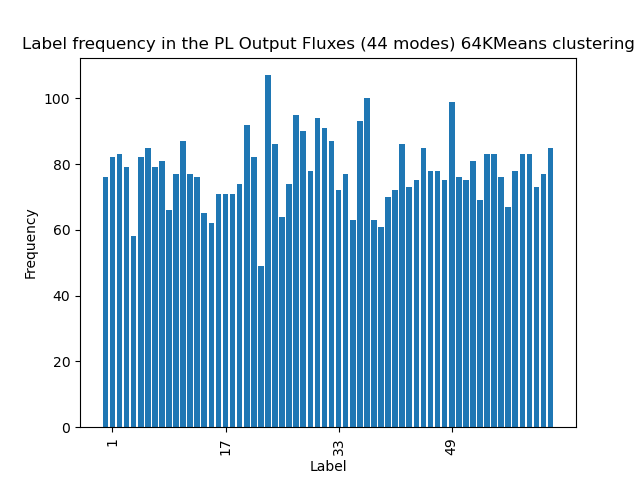
\includegraphics[width=0.2\textwidth]{nmia-ploutputfluxes(44modes)64KMeansdensity.png}}
		\end{figure*}
			
		\begin{figure*}[ht!]
			\centering	
			\subfloat[100KMeans for Zernike coefficients]{%
				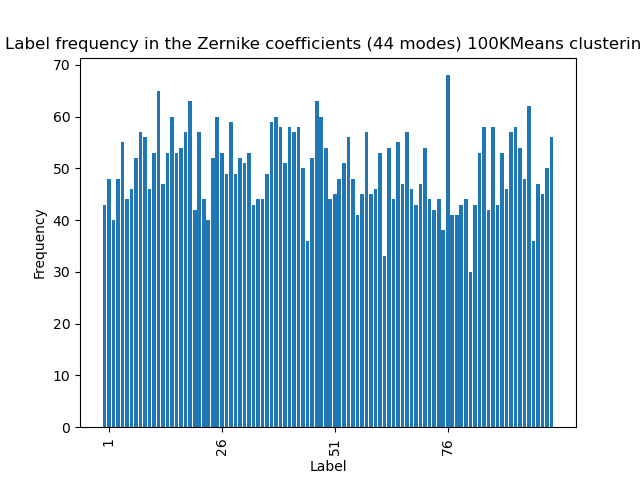
\includegraphics[width=0.2\textwidth]{nmia-zernikecoefficients(44modes)100KMeansdensity.png}}
			\hspace{\fill}
			\subfloat[100KMeans PSF Intensities UMAP]{%
				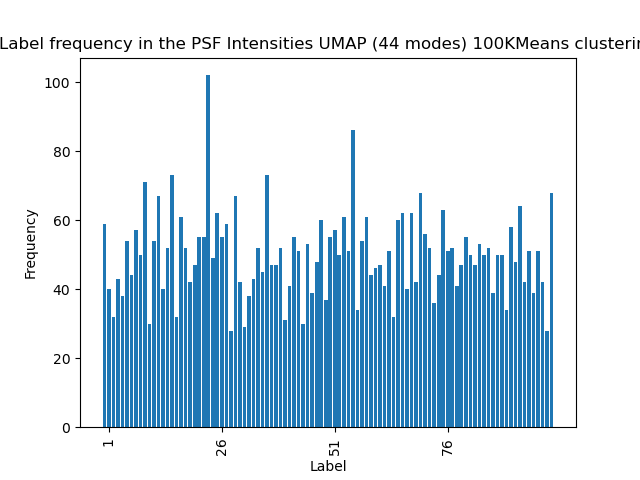
\includegraphics[width=0.2\textwidth]{nmia-psfintensitiesumap(44modes)100KMeansdensity.png}}
			\hspace{\fill}
			\subfloat[100KMeans LP coefficients]{%
				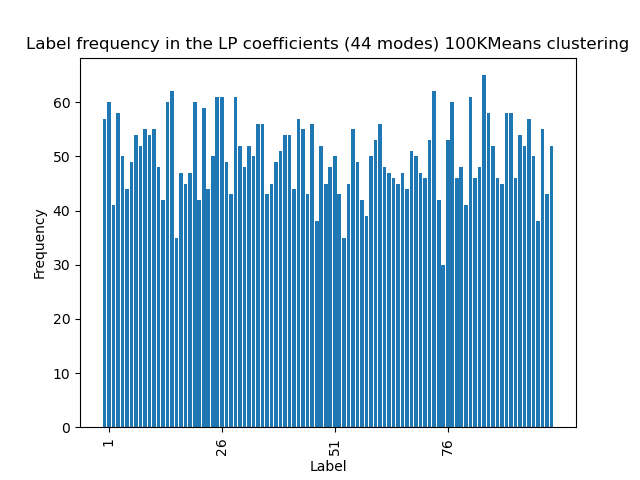
\includegraphics[width=0.2\textwidth]{nmia-lpcoefficients(44modes)100KMeansdensity.png}}
			\hspace{\fill}
			\subfloat[100KMeans Output Fluxes]{%
				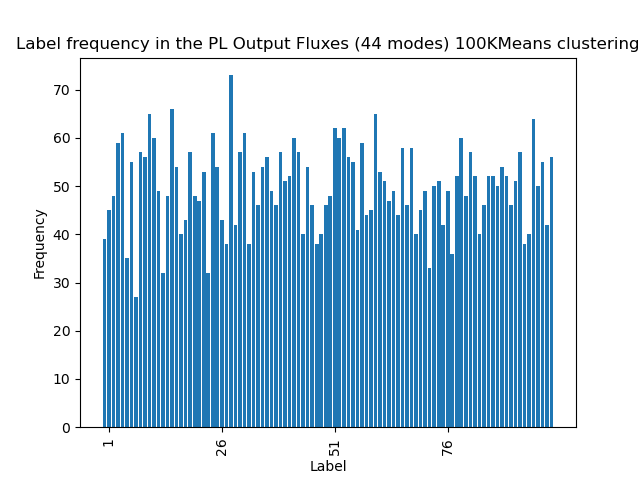
\includegraphics[width=0.2\textwidth]{nmia-ploutputfluxes(44modes)100KMeansdensity.png}}
		\end{figure*}
			
		\begin{figure*}[ht!]
			\centering	
			\subfloat[250KMeans for Zernike coefficients]{%
				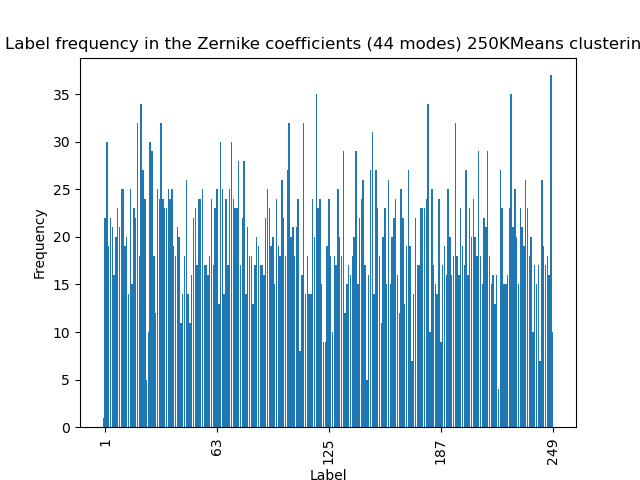
\includegraphics[width=0.2\textwidth]{nmia-zernikecoefficients(44modes)250KMeansdensity.png}}
			\hspace{\fill}
			\subfloat[250KMeans PSF Intensities UMAP]{%
				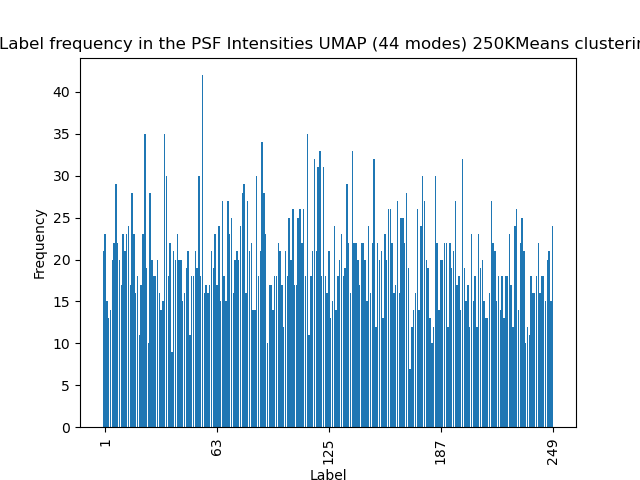
\includegraphics[width=0.2\textwidth]{nmia-psfintensitiesumap(44modes)250KMeansdensity.png}}
			\hspace{\fill}
			\subfloat[250KMeans LP coefficients]{%
				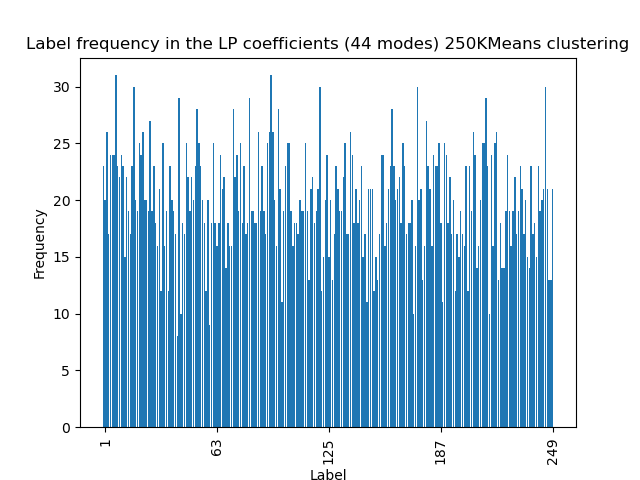
\includegraphics[width=0.2\textwidth]{nmia-lpcoefficients(44modes)250KMeansdensity.png}}
			\hspace{\fill}
			\subfloat[250KMeans Output Fluxes]{%
				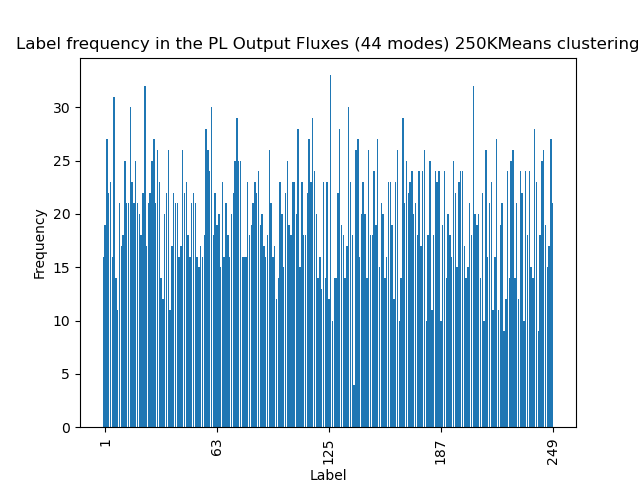
\includegraphics[width=0.2\textwidth]{nmia-ploutputfluxes(44modes)250KMeansdensity.png}}
		\end{figure*}
			
		\begin{figure*}[ht!]
			\centering	
			\subfloat[250KMeans for Zernike coefficients]{%
				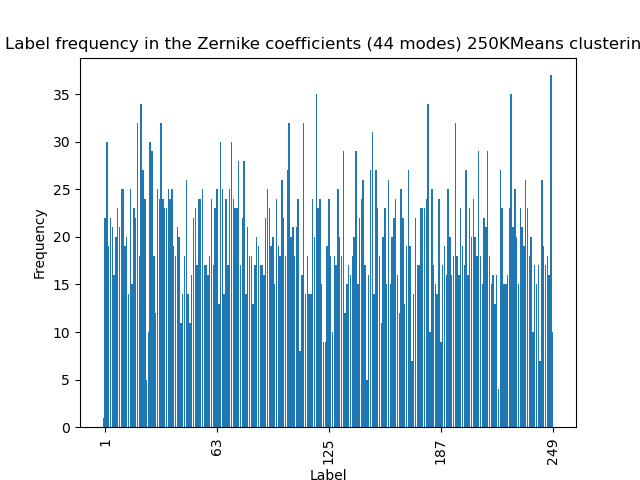
\includegraphics[width=0.2\textwidth]{nmia-zernikecoefficients(44modes)250KMeansdensity.png}}
			\hspace{\fill}
			\subfloat[250KMeans PSF Intensities UMAP]{%
				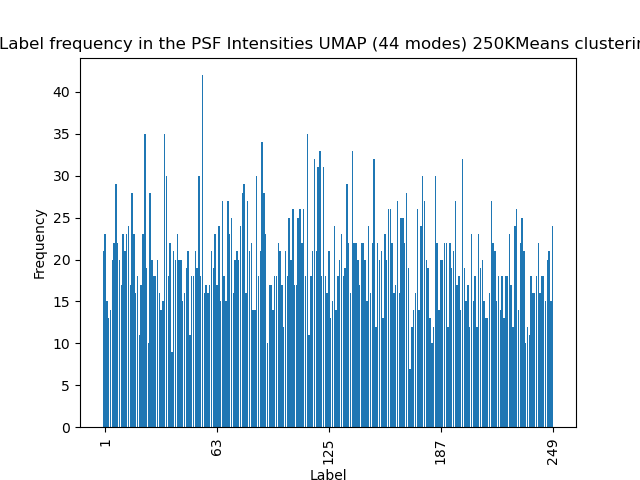
\includegraphics[width=0.2\textwidth]{nmia-psfintensitiesumap(44modes)250KMeansdensity.png}}
			\hspace{\fill}
			\subfloat[250KMeans LP coefficients]{%
				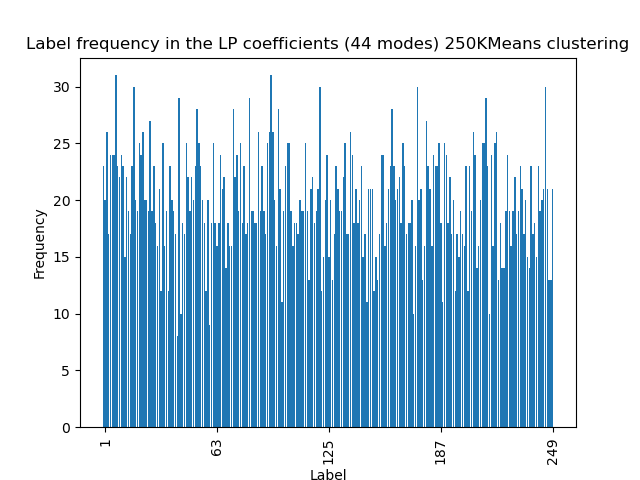
\includegraphics[width=0.2\textwidth]{nmia-lpcoefficients(44modes)250KMeansdensity.png}}
			\hspace{\fill}
			\subfloat[250KMeans Output Fluxes]{%
				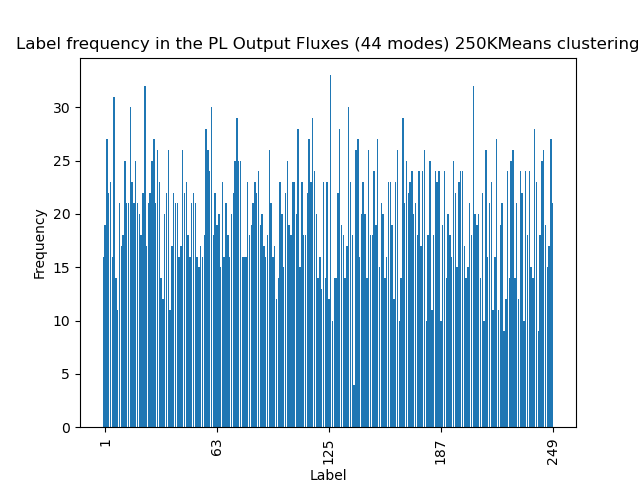
\includegraphics[width=0.2\textwidth]{nmia-ploutputfluxes(44modes)250KMeansdensity.png}}
		\end{figure*}
			
		\begin{figure*}[ht!]
			\centering	
			\subfloat[1000KMeans for Zernike coefficients]{%
				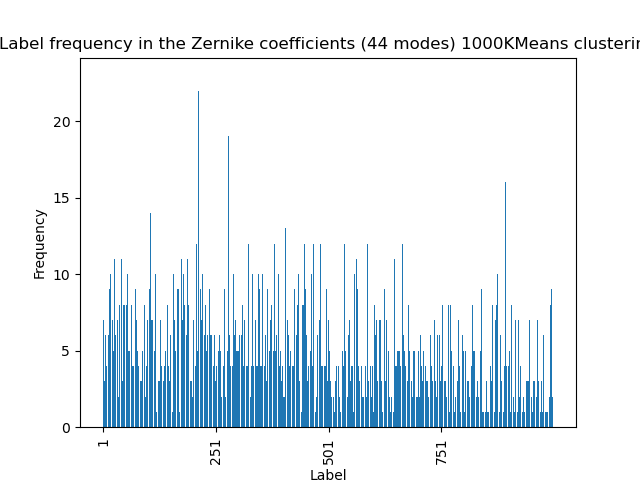
\includegraphics[width=0.2\textwidth]{nmia-zernikecoefficients(44modes)1000KMeansdensity.png}}
			\hspace{\fill}
			\subfloat[250KMeans PSF Intensities UMAP]{%
				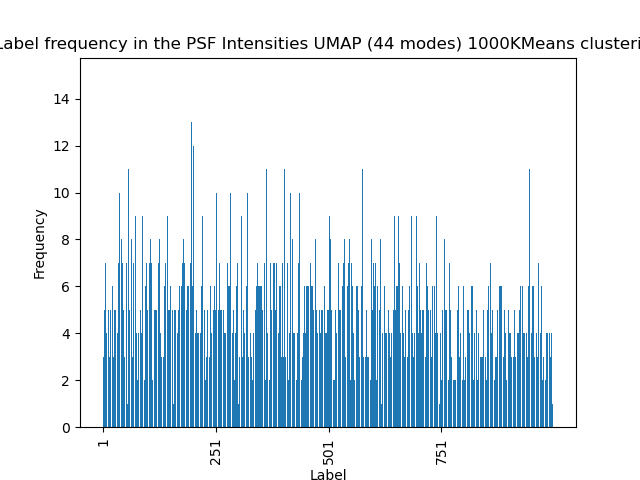
\includegraphics[width=0.2\textwidth]{nmia-psfintensitiesumap(44modes)1000KMeansdensity.png}}
			\hspace{\fill}
			\subfloat[250KMeans LP coefficients]{%
				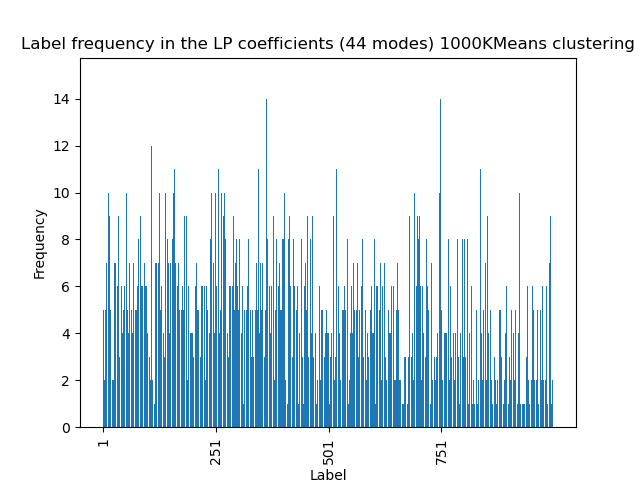
\includegraphics[width=0.2\textwidth]{nmia-lpcoefficients(44modes)1000KMeansdensity.png}}
			\hspace{\fill}
			\subfloat[250KMeans Output Fluxes]{%
				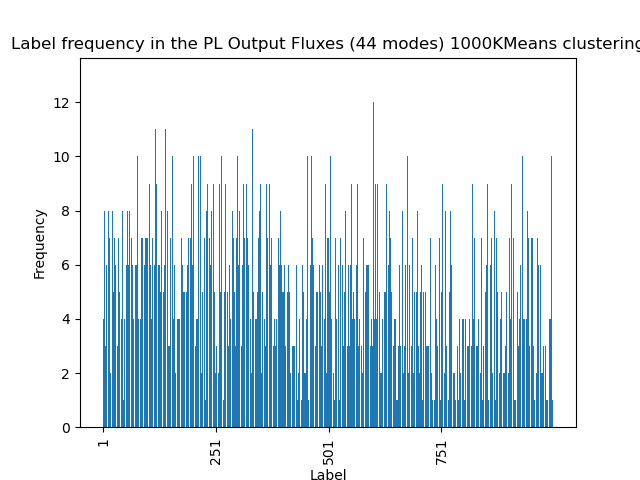
\includegraphics[width=0.2\textwidth]{nmia-ploutputfluxes(44modes)1000KMeansdensity.png}}
		\end{figure*}
		\FloatBarrier